
\section{Propagation}

% Cosmic ray propagating in the galaxy
\subsection{Cosmic rays propagating in the galaxy}
When the accelerated cosmic rays leave the SNRs, they travel through the Galaxy and then interact with the ISM producing secondary cosmic rays. By hadronic production, antiprotons can be generated. Positrons and electrons lose their energy by bremsstrahlung and synchrotron radiation in the interaction collisions. Due to their charge, cosmic rays are scattered on the magneto-hydrodynamic (MHD) waves, so their trajectory is deflected from a straight line. The path of cosmic rays can be described by a diffusion process. The effects of this diffusion, as well as other physical effects, can be quantitatively described by the transport equation \cite{CosmicRayPropagationEquation}:     

\begin{equation}  
\frac{ \partial \psi(\vec{r},p,t)}{\partial t} = q(\vec{r},p,t)  + \vec{\nabla} \cdot  (D_{xx} \vec{\nabla} \psi - \vec{V}\psi) + \frac{\partial}{\partial p}p^2 D_{pp} \frac{\partial}{\partial p} \frac{1}{p^2}\psi - \frac{\partial}{\partial p } \left [ \dot p \psi - \frac{p}{3}(\vec{\nabla} \cdot \vec{V}) \psi \right ] - \frac{1}{\tau_{f}}\psi - \frac{1}{\tau_{r}}\psi
\label{PropagationEquation}
\end{equation}

where $\psi(\vec{r},p,t)$ is the density of cosmic rays at point $\vec{r}$ with momentum p. The terms of the equation describe different physical processes and are explained here:

\begin{itemize}
\item $q(\vec{r},p,t)$ denotes the source term, that includes the primary sources, and the contributions from spallation and decay processes.
\item $D_{xx}$ is the spatial diffusion coefficient that describes the scattering off the magneto-hydrodynamic waves.
\item $\vec{V}$ is the convection velocity. The galactic winds cause an additional convective transport.
\item $D_{pp}$ is the momentum diffusion coefficient. Apart from the spatial diffusion process, charged particles traveling in MHD waves undergo stochastic re-acceleration that can be described by the momentum diffusion coefficient.
%\item $\vec{\nabla} \cdot \vec{V}$ denotes the adiabatic momentum change, this term is caused by scattering off inhomogeneities of the magnetic field. 
\item $\vec{\nabla} \cdot \vec{V}$ denotes the adiabatic momentum change, this term is the work against the pressure of the interstellar gas.
\item $\tau_{f}$ and $\tau_{r}$ are the time scales of fragmentation and radioactive decay respectively.
\end{itemize}

For each particle type a propagation equation is used, leading to a very complex system of differential equations. To solve these equations analytically is impossible, therefore numerical calculations are more practical, like Monte-Carlo based approaches. Software numerical tools that are widely used to obtain the solution of the transport equation are the following: GALPROP \cite{GALPROP}, USINE \cite{USINE}, and DRAGON \cite{DRAGON}.  \par

Alternatively, it is possible to solve simplified approximations of Eq. \ref{PropagationEquation}. The basic assumption is that the galaxy is a box where particles can freely propagate while undergoing only elastic scattering. In this case, the density of cosmic rays does not depend on the location within the box. At the edge of the box, the particles are reflected with a probability $1-P_\mathrm{esc}$, and the $P_\mathrm{esc}$ is the probability of escaping to the outside of the box. As a consequence, the diffusion term can be replaced by escape time $\tau_\mathrm{esc}$. With this assumption, the transport equation can be simplified as:

\begin{equation}  
\frac{ \partial \psi(\vec{r},p,t)}{\partial t} = \psi_{0}(p) \cdot \delta(t) - \frac{\psi(p,t)}{\tau_\mathrm{esc}}
\end{equation}

where $\tau_{esc}$ is escape time which represents the constant escape probability, $\psi_{0}(p)$ is the injection homogenous source of particles at the time t=0. This simplified approximation is called the Leaky-Box model \cite{LeakyBoxModel} and its solution is:

\begin{equation}  
\psi(p,t) = \psi_{0}(p)\rm{exp}(-\frac{t}{\tau_\mathrm{esc}}) 
\end{equation}


% Cosmic ray propagating in the heliosphere
\subsection{Cosmic ray propagating in the heliosphere}
%% Heliosphere: sun --> solar wind --> HMF and HCS --> termination shock
The Sun is continuously ejecting from its upper atmosphere a stream of charged particles when the energy of those particles surpasses the escape limit, this form the solar wind \cite{SolarWind1, SolarWind2}. The solar wind plasma drags outwards the solar magnetic field forming the HMF \cite{HeliosphericMagneticField}. Because of the rotation of the Sun, the HMF has a spiral shape which is called Parker spiral, and the shape of the HMF is changing with the Sun's activity. The opposite polarity of HMF is separated by the heliospheric current sheet (HCS). The charged particles of the solar wind reach speeds of around 400 km/s, meaning they are faster than the speed of the magnetosonic wave, therefore they are supersonic. After traveling for some distance and encountering the interstellar medium, the speed of the solar wind abruptly decelerates and becomes subsonic at the termination shock \cite{HeliospherePaper}. Figure \ref{Heliosphere} shows a diagram of the heliosphere. The Voyager 1 probe became the first spacecraft to cross the termination shock in 2004 and later in 2012 to encounter the heliopause \cite{Voyager1Paper}. As shown in Figure \ref{Voyager1}, the solar wind particle rate dramatically decreases after reaching the outer border of the heliosphere.

\begin{figure} \centering   
\subfigure[] { \label{Heliosphere}    
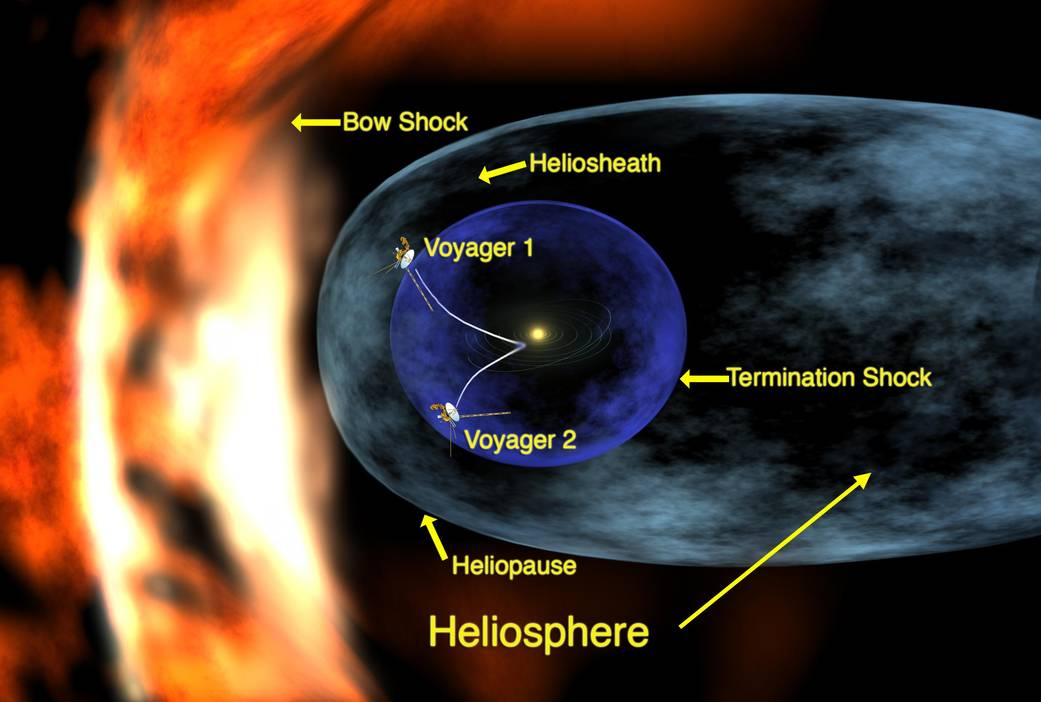
\includegraphics[width=0.47\columnwidth, height=0.26\textheight]{Figures/chapter2/Propagations/Heliosphere.jpg} 
}    
\subfigure[] { \label{Voyager1}    
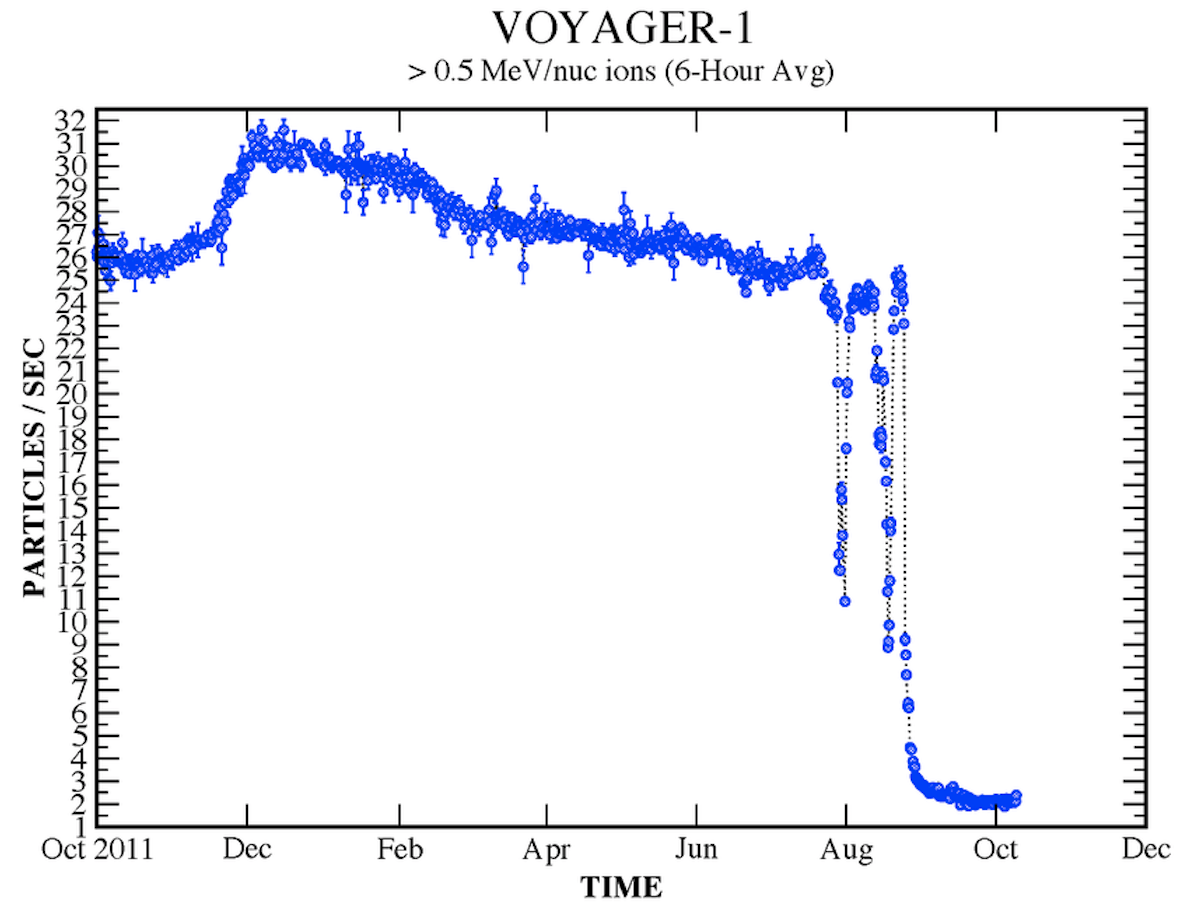
\includegraphics[width=0.47\columnwidth, height=0.26\textheight]{Figures/chapter2/Propagations/Voyager1.png}    
}    
\caption[Heliosphere and Particle rate detected by Voyager 1.]{a) Diagram of the heliosphere. Credit: NASA/Walt Feimer; b) Particle rate detected by Voyager 1 (from October 2011 through October 2012) \cite{WikiVoyager1ReachHeliosphere}.}     
\end{figure}

% sunspot difination -> sun rotation --> polartiy reverse 11 years (22 years cycle) --> the HMF shape change with sun activity
Sunspot is a spot that looks darker than the surrounding areas on the Sun's photosphere, which represents solar activity. During the solar maximum, the number of sunspots reaches the maximum and the polarity of the HMF reverses. The sunspot number changes in a cycle of 11 years. Considering the polarity, a full cycle of the Sun's activity is 22 years \cite{SolarCycle}. The solar cycles have been counted since 1755 and now we are in solar cycle 25 \cite{SolarCycleFirstObservation1, SolarCycleFirstObservation2}. \par


% propagation in the heliosphere 
When galactic cosmic rays enter the solar system, they travel through the heliosphere first before reaching the Earth. The propagation process is similar to the propagation in the galaxy but the diffusion coefficient is orders of magnitude smaller. Since the full transportation equation can not be solved analytically, a simplified model proposed in \cite{ForceFieldApproximationPaper} is usually used and it describes the process as the diffusion through the HMF. In this model, under the force-field approximation, an analytical solution of the one-dimensional steady-state equation is derived, which relates the GCR spectrum measured at Earth $J$ and in the local interstellar space  $J_\mathrm{LIS}$:  

\begin{equation}
J(T_{\rm{E}}) = \frac{T_{\rm{E}}(T_{\rm{E}}+2M)}{T_{\rm{HP}}(T_{\rm{HP}}+2M)} J_\mathrm{LIS}(T_{\rm{HP}})
\end{equation}

where the $M$ is the particle mass, $T_{\rm{E}}$ and $T_{\rm{HP}}$ are the kinetic energies of the particle at Earth and at the heliopause. $T_{\rm{HP}}=T_{\rm{E}} + Z \phi$, and $\phi$ is called modulation potential, which depends on the solar wind speed and the diffusion coefficient. Since the solar activity and the physical status of the heliopause vary following the 22-year cycle, the measured GCR spectrum at Earth also shows a variation of the 22-year cycle. This is called solar modulation. 

%   sunspot vs CRs: anti-correlated
\begin{figure}[t]
\centering
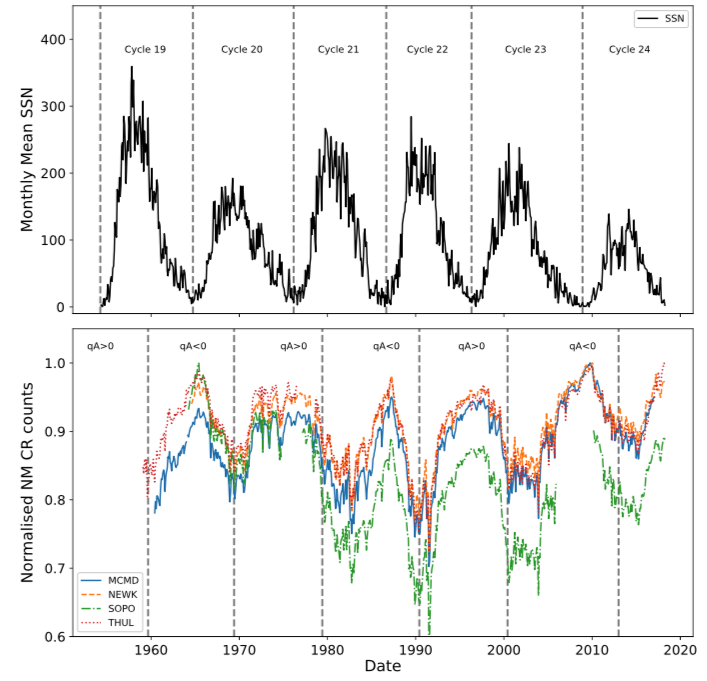
\includegraphics[width=0.80\textwidth, height=0.5\textheight]{Figures/chapter2/Propagations/NeutronMonitor.png}
\caption[Cosmic rays intensity and Monthly mean sunspot numbers.]{Bottom figure: The cosmic rays (CR) intensity recorded by neutron monitor (NM) counts from four different stations (MCMD = McMurdo, NEWK = Newark, SOPO = South Pole, THUL = Thule). The vertical lines show the approximations of epochs of solar magnetic-field polarity reversals and qA is the solar polarity. Top figure: Monthly mean sunspot numbers (SSN) over the latest six solar cycles. The vertical lines show the beginning of each solar cycle. The figure is taken from \cite{NeutronMonitor}. }
\label{NeutronMonitor}
\end{figure}

In the figure \ref{NeutronMonitor}, the different ground-based cosmic neutron measurements and the monthly mean sunspot numbers are shown. The cosmic neutron counts show the intensity of hadronic cosmic rays, which indicate the measured cosmic rays at Earth. The sunspot numbers are correlated to solar activity. When the GCRs enter the solar system, they interact with the solar wind and magnetic fields. A large solar activity reduces the cosmic rays and vice versa. Therefore, the sunspot numbers and the cosmic neutron counts are anti-correlated. By measuring the cosmic ray flux over a long period of time, the impact of solar activity can be studied. Until recently, the only continuous cosmic ray flux measurements over a long period of time have been performed only for the dominant components of the cosmic spectrum like protons, helium, electron or neutrons produced in cascades in the Earth’s atmosphere. There is no continuous measurement of rare cosmic ray components like antiproton. Since the AMS-02 experiment has been collecting cosmic data for 10 years, the first time-dependent antiproton measurement can be achieved.  \par 

% Drift--->Particle Sign Different
Due to the sign of charged particles, they drift differently in different polarities. For example, in positive polarity, the positively charged particles drift toward the Sun from the heliospheric poles and outwards to Earth. While the negatively charged particles drift arriving at Earth inwards along the HCS. This leads to different diffusion processes in the heliosphere. This charge-dependent modulation results in a different behavior between antiprotons and protons, furthermore, the antiproton to proton flux ratio behaves differently in opposite polarity periods. Similarly, positron and electron also behave differently due to opposite charge signs. In the time-dependent positron to electron flux ratio measurement by AMS-02 \cite{AMSElectronPositronPaper}, this can be observed. Also, the reversal of polarity is not easy to be determined clearly. The measurement of the positron to electron flux ratio can provide information about the reversal period.


% 太阳的结构,可以形象的称之为“里三层、外三层”模型。里三层,是指太阳内部的核反应区(日核)Core、辐射区Radiative zone、对流区(对流层)Convective zone;外三层,是指太阳大气的光球层Photosphere、色球层Chromosphere、日冕层Corona。
% 太阳磁场主要在太阳大气层 - 光球Photosphere、色球Chromosphere 和 日冕Corona低层中
% 太阳磁场还有周期性的磁场反转,与黑子的出现地点有所关连,黑子的出现地点会从太阳极区渐渐移往赤道地区,可以用蝴蝶图来表示,呈现约11年的周期变化,太阳磁场也是约每11年反转一次



